\chapter{Architectures and Frameworks}
\label{chap:ch3}

\section{Mobile application}
\label{sec:ch3sec1}

\par We have decided to write the entire mobile application in Kotlin and use the Model-View-ViewModel (MVVM) architecture in a combination with Koin as our dependency injection tool. To accomplish the reading of data from the bracelets we will use the default NfcAdapter provided by Android as it is a reliable way to achieve our goal of retrieving the information from those tags.

MVVM is our go for the mobile application architecture because it is currently considered to be the best choice in the case of Android applications since it is easy to adapt in most scenarios. This architecture helps us write more reusable code (if used right) and gives us flexibility in changing our user interface without necessarily having to refactor other logic in the code base.

A good and comprehensive definition of the MVVM theory can be found in \cite{anderson2012model}, and it states: "At the heart of the MVVM design pattern is the separation of a view’s logic from its look. Instead of having a mass of code in a View’s code-behind, much of this code will be extracted out into a ViewModel class separated from the View itself. This ViewModel class will then expose data and operations publicly for one or more Views to consume. The result of this will be that the view should have very little code-behind. You can then use data bindings and commands/behaviors as the glue to connect the View and the ViewModel together."

The architecture consists of three layers: Model, View and ViewModel, which we are going to tackle separately and it can be seen in figure \ref{fig:mvvm}. An example of how the architecture is used in our project can be seen in figure \ref{fig:mvvm-project-example}.

\begin{figure}
\centering
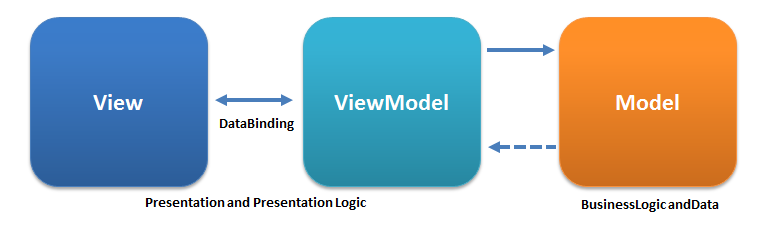
\includegraphics[width=\textwidth]{figures/fig_3_1.png}
\caption{The MVVM architecture \cite{mvvmPattern}}
\label{fig:mvvm}
\end{figure}

\begin{figure}
\centering
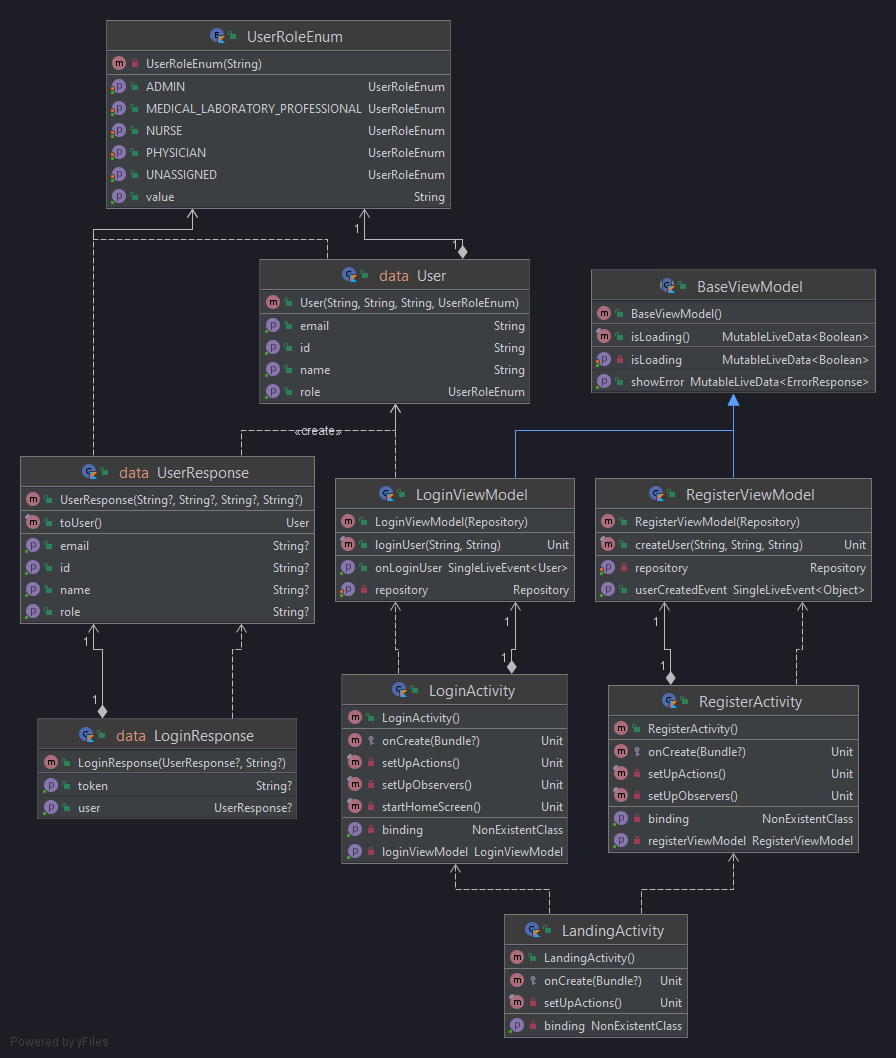
\includegraphics[width=\textwidth]{figures/mvvm_project_example.png}
\caption{The UML class diagram for the Sign Up and Sign In use-cases to exemplify the MVVM architecture of the project}
\label{fig:mvvm-project-example}
\end{figure}

\subsection{The Model}
\label{subsec:ch3sec1subsec1}

\par Let us begin with the basic building block which is a key component for all applications, concretely: information and data. Those are stored in the model. The model is basically the domain object and it represents the actual data and/or information that is used throughout the application. A basic example of such a model could be a user, which would contain an ID, a name, an email address and an assigned role, as seen in figure \ref{fig:user-uml}.

\begin{figure}
\centering
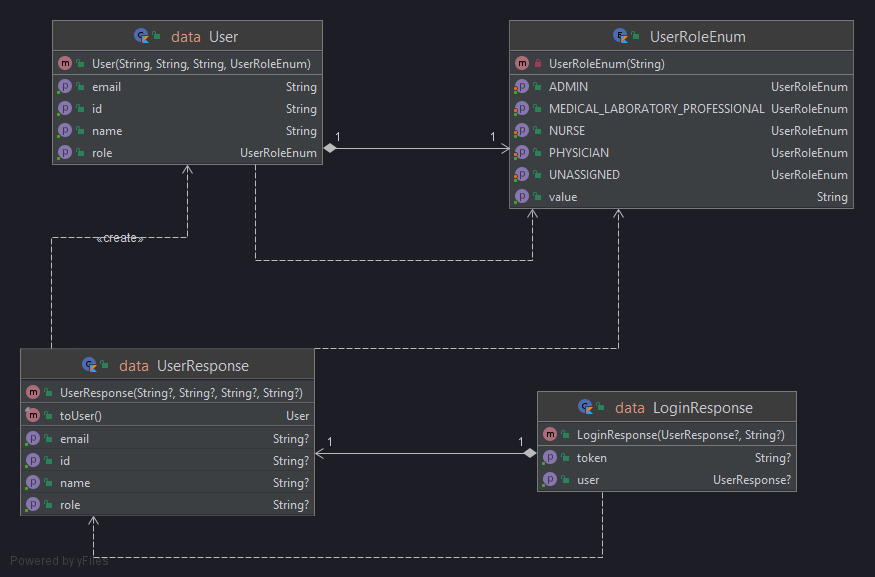
\includegraphics[width=\textwidth]{figures/user_uml.png}
\caption{The UML class diagram for the User model}
\label{fig:user-uml}
\end{figure}

The most important thing about the model that we should keep in mind is that it holds the actual data and information, but not the logic or services that process it. The model should not be responsible for fetching data from a server or formatting text to display on the screen. However there are some exceptions where some models do contain some business logic like validations, but typically this should be separated from the model.

\subsection{The View}
\label{subsec:ch3sec1subsec2}

\par The view is basically the only interactable part of our application to the end user, the user interface, or the way we present our data. The view manipulates the data and formats it in order to make it easier to be consumed by the end user. As a quick example we have a date that might be stored as a timestamp that looks something like "2021-05-31T01:48:52Z" in our model, while for the end user it will be displayed as the year, month, day, hour, minute and second in their specific timezone. Also, a view can have associated behaviors with it, like for example accepting some user input through input text fields for your email and password. It manages inputs which in the end change properties in the model.

As opposed to some other architectures, the view in MVVM is active, which means that it doesn't completely turn over the control of its state to the viewmodel / controller / presenter. The view is responsible of its own events, contains behaviors and data-bindings which in the end needs to know about the underlying structure (the model and the viewmodel). Sure the events might be mapped to some commands or method calls, but the view is still responsible, in the MVVM architecture, of handling the events that belong to it.

However, an important note is that the view is still not responsible of maintaining its state, it should synchronize it with the viewmodel, about which we will talk next.

\subsection{The ViewModel}
\label{subsec:ch3sec1subsec3}

\par The viewmodel is our controller, or presenter if you want. It is the key piece of the architecture that helps keeping the view separated form the model. In this way the model does not need to be aware of the users view of the data, and instead it only holds the information, while the view holds the formatted information. The viewmodel behaves like a link between them.

The viewmodel will maybe interact with a service in order to retrieve the model in order to format the information and pass it to the view, or it might take an input from the view in order to pass it to the model. It also exposes methods, commands, and other points that help maintain the state of the view, manipulate the model as the result of actions on the view, and trigger events in the view itself. \cite{viewmodel}

\section{Server application}
\label{subsec:ch3sec2}

\par To write our server applications we have decided to use the new Kotlin for servers plugin created by JetBrains called Ktor. As for the database we have chosen PostgreSQL as there are easy integrations between it and Ktor made possible by some frameworks provided by JetBrains.

\subsection{Ktor}
\label{subsec:ch3sec2subsec1}

\par Ktor is an asynchronous framework for creating microservices, web applications, and more. It’s fun, free, and open source. \cite{ktor}

First of all we have chosen to use Ktor because of our familiarity with Kotlin, coming from a mobile development background. However, that was not the only reason. Ktor provides us with a very simple way of creating a server by taking the responsability of running asynchronous tasks in its own hands.

The syntax in Ktor is very simple and simple to understand. It uses some install statements in order to build some components by default, taking a lot of work off of our shoulders and removing a lot of so called boiler-plate code from the project, some examples would be the default headers that should be attached to every response, the error handling and the JSON content negotiation. The code for all of those can be seen in figure \ref{fig:install-statements}.

\begin{figure}
\centering
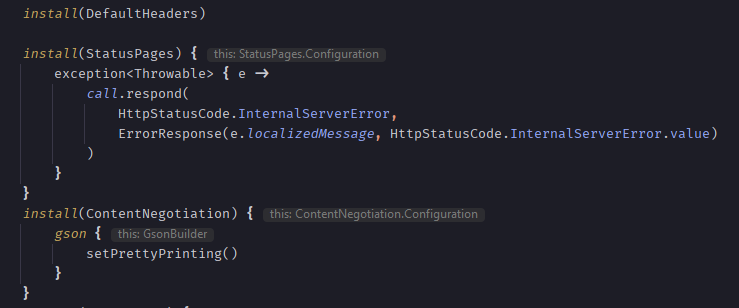
\includegraphics[width=\textwidth]{figures/install_statements_snippet.png}
\caption{Ktor install statements code snippet}
\label{fig:install-statements}
\end{figure}

\subsection{PostgreSQL}
\label{subsec:ch3sec2subsec2}

\par The reason for which we have chosen PostgreSQL is because it is very easy to be integrated with Ktor by only using three (3) main frameworks. Those frameworks are the following: the Exposed Object-relational mapping (ORM) library, the Java Database Connectivity (JDBC) Connection Pool HikariCP library and the Java Database Connectivity (JDBC) Connector for PostgreSQL.

The Exposed library is used in order to map the database tables into Ktor readable objects that can be interrogated easily with a Kotlin-like syntax. Take for example the getUserById method from figure \ref{fig:getUserById}, where Users represents a so called UUID (Universally Unique Identifier) Table, a table for which the IDs are auto-generated as UUIDs (figure \ref{fig:users-table}).

\begin{figure}
\centering
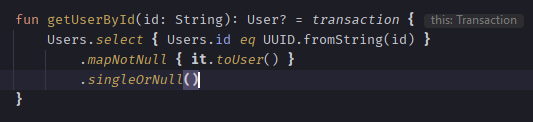
\includegraphics[width=0.75\textwidth]{figures/get_user_by_id.png}
\caption{Exposed syntax example for interrogating the database}
\label{fig:getUserById}
\end{figure}

\begin{figure}
\centering
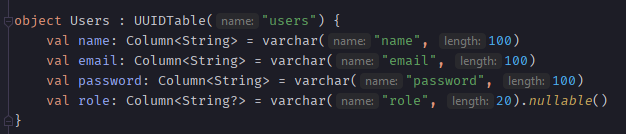
\includegraphics[width=0.75\textwidth]{figures/users_table_example.png}
\caption{Exposed syntax example for the Users table definition}
\label{fig:users-table}
\end{figure}

The Hikari Connection Pool library provides us with an easy way to configure the connection to the actual database. It only requires a configuration file which we pass to its constructor and we are good to go.

The PostgreSQL library is only included for support in order to connect to the database using Hikari.